
\section{Definici�n del Problema}
\begin{frame}{Definici�n del Problema}

\framesubtitle{Reconocimiento de Actividades Humanas}
\begin{center}
Determinar las acciones o comportamientos de uno o m�s individuos
a partir de datos ambiguos capturados por sensores situados en el
entorno.
\par\end{center}

\end{frame}
%
\begin{frame}[<+->]{Definici�n del Problema}

\setbeamercovered{transparent}

\framesubtitle{�Que es HAR?}
\begin{itemize}
\item Es un t�pico de investigaci�n multidisciplinario para dise�ar algoritmos
para:
\begin{itemize}
\item Capturar movimientos de uno o m�s individuos en interacci�n con su
entorno 
\item Realizar el aprendizaje e inferencia
\item Proveer informaci�n de contexto 
\end{itemize}
\end{itemize}
\begin{center}
\visible<5>{\begin{center}
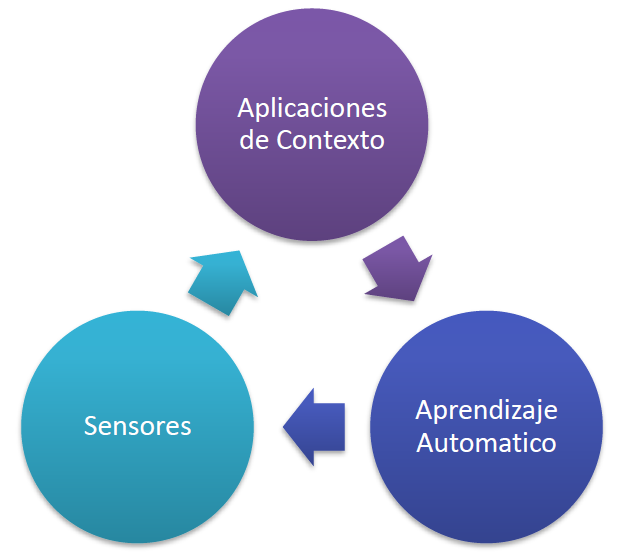
\includegraphics[width=4.5cm]{intro/graphics/areas2}
\par\end{center}}
\par\end{center}
\end{frame}

